\chapter{Setting the scene: finding slippages}
\label{ch:4}

\section{Introduction}
\label{sec:4-intro}

In the previous chapter, I detailed my methodological approach, focusing on the intersections of ethnography, action, and design, and the tensions of doing and writing about research with young people who are oppressed or who have experienced trauma. In the rest of this thesis, I explore what living and working in the care system is like under austerity-intensified capitalist realism, and detail how speculative design methods can support experimental action against the hegemony of capitalist realism. 

In this chapter, I introduce The Charity, its many projects, and the people that I came to know through those projects. As explained in the previous chapter, The Charity is a composite of the organisations I have worked with over the past four years, constructed to avoid damaging the reputation of any of my partner organisations. Throughout this chapter, I "follow [my] ethnographer’s nose twitch" (after \cite{leigh_star_this_2010}), detailing my initial encounters with different people within The Charity and paying attention to my intuition about things that feel amiss. The chapter is structured around three moments in which my attention was brought towards a `slippage' \citep{cutting_making_2021} that was occurring, between the purported values or practice of the people I was working with and what was \textit{actually} happening. In the following two chapters, I will introduce the theory of justification practices, which describes the changes in experiences, affects and practices that have been brought about in the care system due to austerity-intensified capitalist realism. The slippages described in this chapter detail my growing awareness of what I later refer to as justification practices.

\section{Introducing The Charity}

The Charity is a national organisation working across all parts of the UK, and are devoted to work with children and young people that they consider to be vulnerable, with a history of charitable work that goes back as far as the 19th Century. Where possible, they try to empower their teams and projects across the country to make decisions for themselves, as far as is possible. A project being run by The Charity in the Lake District, for example, can be vastly different to one that is running in Bristol, as The Charity values local control and local decision-making; except when they don’t, like when some organisational change means that the entire composition of the organisation has to change. These changes never full take hold, but this tension between central control and local autonomy are a constant for The Charity.

The Charity is funded in a number of ways. Much of their work is commissioned—normally by a local authority outsourcing some of their statutory responsibilities—but other work is grant-funded, giving The Charity an opportunity to fund research or develop new approaches to working with young people perceived to be vulnerable. On top of this, some work is also funded by "unrestricted finance"— money donated by members of the public that allows them to work on `innovative' projects and strategically prioritise certain areas of work. These three different funding streams give rise to distinct working experiences. People working on commissioned projects might find that they are only allowed to deliver work that is explicitly within the project's contract. Grant-funded projects may appear to have more flexibility, but the strict bureaucracy around evaluation and reporting often means their hands are just as tied as commissioned project workers. Projects funded by unrestricted finance easily have the largest degree of flexibility—but their `strategic' nature often means they have to operate under the watchful gaze of senior central teams. 

As a result, there are a variety of types of workers within The Charity. The majority of people I worked with in The Charity tended to be youth workers or social workers, yet all sorts of workers exist in such a vast organisation. There are researchers, HR, admin and finance staff, business managers, mental health workers, and ex-civil servants in senior managerial roles. Most of the people I worked closely with, though, came from conventional charity backgrounds, either primarily having worked in a helping or caring profession, or making a career change at some point to do that. Some were professionally trained, pursuing social work qualifications at university before joining The Charity, whilst others did their training on the job, pursuing youth work qualifications through working with The Charity, or joining whilst on placement from their course. 

Although other areas and projects within The Charity show up occasionally within this thesis, I  worked primarily with three main projects: Small Steps, Building Bridges, and Seabird. Small Steps is a project focused on developing research and policy to support young people with experience of homelessness in the North of England. Building Bridges is a project based across the country, focused on supporting care-experienced young people to identify ways that they want to change the care system and providing them with resources to work towards making those changes. Finally, Seabird is a project providing youth and social work services for care-experienced young people in the South of England. All three projects had some level of awareness of each other, but there was not necessarily a huge degree of interaction between them. In the rest of this chapter, I will introduce you to members of each project in turn, and the slippages that gradually became apparent as I spent more time with them. 

\section{Noticing slippages}

Along with introducing you to the members of each project I have worked with, I want to show how each of these projects began to make apparent the invisible network of power relations that they operated within. To do this, I will be using the concept of slippages. \citet{fanon_black_1986} first detailed slippages in reference to the "ethical slippage" (\textit{un glissement ethique}) that described how the moral values of white France were able to take hold in the consciousness of Black Martinicans. The concept of slippages allowed Fanon to surface how the values and priorities of one world could be transported to another world in which they did not fit, resulting in oppression. Martinicans came to inherit the colonial French value system that "black is bad, immoral, and sinful, while white is good, virtuous, and pure" \citep[p. 11]{sullivan_ethical_2004}, considering whiteness to be equated with morality. These values slip into subconscious thought and action, often diffused through media, and operate without much conscious attention being brought towards them. 

My use of the concept builds on Fanon's. In my rendering \citep{cutting_making_2021}, slippages refer to the moments that we recognise our current actions are operating from a different valueset than our own. In research, this is particularly critical for people using ethnographic or observation-based methods, as noticing a slippage is often what helps us to recognise the nature of the phenomenon we are researching. You may think that you are researching one thing, but suddenly you notice everything feels different and your attention is redirected. You might notice a widening bifurcation between a person or project's values and actions. You might find yourself pulled into a worldview, imaginary, or ideology that is not your own. You may just as easily slip back, but once you have seen the presence of this other worldview (and indeed, the other world that is constructed by this worldview), then it is due diligence to follow the phenomenon. Slippages are Leigh Star's "ethnographer's nose twitch" \citep[p. 610]{leigh_star_this_2010}, an act of noticing that allows the researcher to become more keenly aware of the affects that participants are constantly experiencing and the environments they must navigate. 

In this section, I describe slippages happening across the three different projects I worked with, and use these as an opportunity to explain the dynamics of the project, the people involved with it, and the slippage that underpinned my research with them. Small Steps made me aware of \textit{how} austerity-intensified capitalist realism begins to affect projects and organizations. Then,  Building Bridges me aware of how managers feel powerless, despite having freedom to choose how they act. Finally, with Seabird, I began to realise how these mindsets become embedded within projects and workers, indicating some of what I will later identify as justification practices. 

\subsection{From peer support to product}
Small Steps was the first project by The Charity that I was introduced to. When I first meet them in 2018, they are a newly-independent project, just starting to find their feet with their own small team. Until 2017, they had been hosted within another project in The Charity, but it became apparent that they needed to spin off into their own project if they wanted to continue their work on research-led policy advocacy for young people with experience of homelessness. Their staff consists of Shelly, the Director; Colin, the Regional Project Officer; Randall, the Communications Intern; and Ronnie, the Fundraising Officer (these are also shown in table \ref{tab:small-steps-participants} for ease of reference). I soon come to learn that these job titles are incredibly malleable—Ronnie mostly does the team's finance and admin; Shelly does most of the grant writing; Colin does \textit{everything} that involves direct work with young people and Randall is `encouraged' to do more than he's meant to because Shelly thinks it will help him after his degree, which he is in the middle of. They also have a few infrequent volunteers and projects run with volunteers from a local university. 
\begin{table}[h!]
\centering
\begin{tabular}{|l|l|} \hline 
\textbf{Name (pseudonym)} & \textbf{Role}                    \\ \hline 
Shelly& Director\\ \hline 
Colin& Regional Project Officer\\ \hline 
Randall& Communications Intern\\ \hline 
Ronnie& Fundraising Officer\\\hline\end{tabular}

\caption{A list of participants from the Small Steps project.}
\label{tab:small-steps-participants}
\end{table}

I first meet Small Steps when they contact my research group: they have recently received some funding to redesign their website and develop an app to increase access to their resources for young people who might be at risk of becoming homeless. Their then-website was mostly geared towards professionals, but they found through their website's analytics that many of their users were much younger, and therefore might be a young person at risk of homelessness seeking support or resources. They heard that my research group is known for helping charities out with digital projects, and after an initial meeting, it's agreed that we will work together exploring the design of digital peer support systems for young people with experience of homelessness. Randall and Colin are excited about the potentials of something less transactional than the original project idea, but are sceptical as to whether Shelly will agree. 

I meet Shelly at Small Steps' office across town the next day (shown in figure \ref{fig:small-steps}. Their offices are my first taste of the world of charities that support young people perceived to be vulnerable. In an otherwise grey and impersonal office, colourful memories of previous projects line the walls. One is a mosaic, the word "HOME" made up of the word "hope" written over and over. Another is a linocut print of a home torn in two. Another, a collage of letters cut from magazines, reading "family is as noisy as a traffic jam". A whiteboard containing the team's schedule looms over the room, whilst stacks of paper fill every free nook and cranny of the office. Every project office I enter after this is similar: grey walls strewn with memories of previous projects and paperwork bursting at the seams. Shelly greets me enthusiastically, shares a little of the history of the organization with me, and we get to talking about my project. She likes the idea of exploring digital peer support, but doesn't quite see how it helps Small Steps right now. She's willing to give it a go, but has worries about moderation, about things "going bad", and wants to ensure that the young people using the platform aren't too "risky". A pattern continues over the next few months: Colin, Randall and I agree something important concerning the project, we tell Shelly about it, she agrees, and then a week later wants us to do something entirely different. At one point, we agree that data privacy and security will be integral throughout the project, as we want the young people we're working with to feel comfortable that they have control over their own information. After a few weeks, Shelly begins making a case that we should ask for consent to allow their information to be included in the project's research:
\begin{quote}
It's just too good an opportunity to miss. This could really help us to get really young-person informed research.
\end{quote}
One evening, after I helped Colin out with a young people's workshop he'd been running, I checked in with him. "You look exhausted, mate, you alright?". He replied:
\begin{quote}
Aye, it's fine, it's just... Shelly's got me doing everything, man. I'm here, there and everywhere, and she wants us to do a blog about the workshops I've been running, and I've still gotta be up and down the M5 every week and there's just not enough time, y'know?
\end{quote}
"Yeah, that sounds like a lot. I noticed you've been doing loads lately", I responded. He looked resigned.
\begin{quote}
It'll be fine, it's just—you know, you need to be careful. She means the best but Shelly'll have every pound of flesh she can get. You'll be next!    
\end{quote}

\begin{figure}
    \centering
    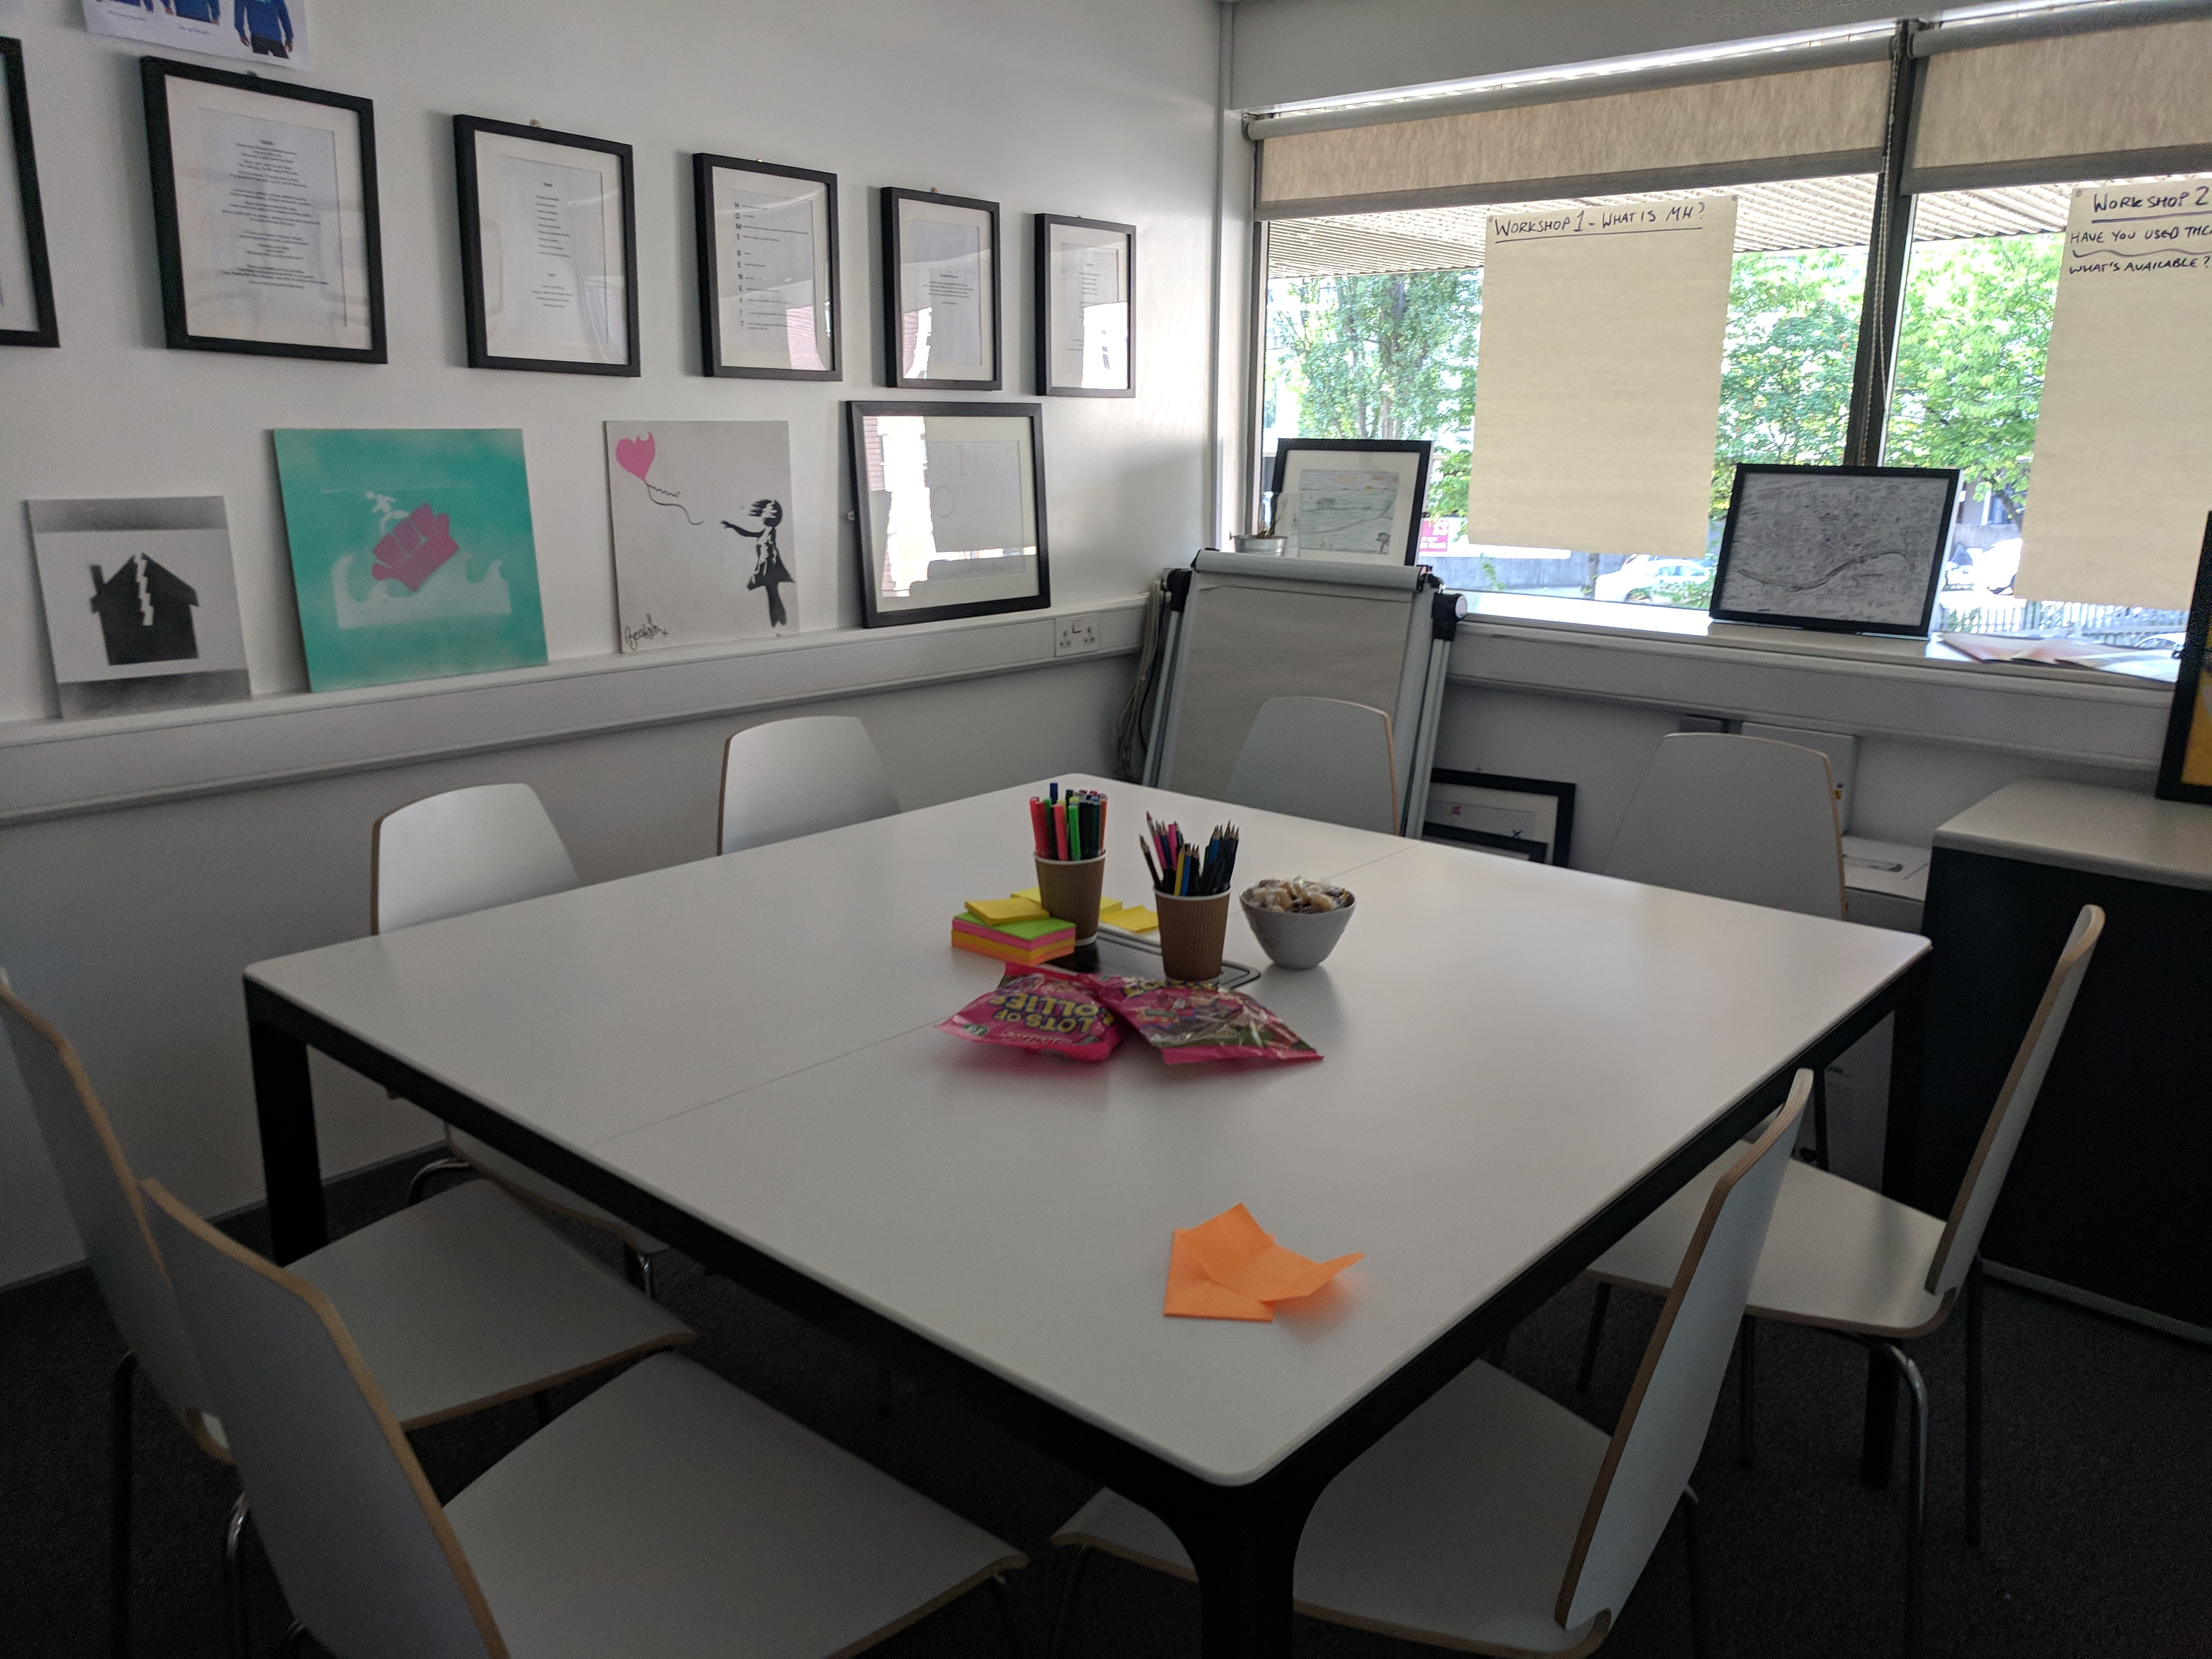
\includegraphics[width=1\linewidth]{Images/3/small-steps.jpg}
    \caption{The meeting room in Small Steps' offices.}
    \label{fig:small-steps}
\end{figure}

I knew what Colin meant. It had felt like Shelly had been wanting more and more from me lately. First it was borrowing some equipment from the research group, which I was happy to help with. Then it was asking me if I would do some evaluation for them on their new project. The boundaries of research like this are so malleable, so you never know when too much is too much. Is it building rapport? Is it helping the organisation? Is it necessary for the work to go further? I knew it had started to go too far, though, when Shelly had asked me to develop a funding bid for the organisation. It was a fund that I had access to because of my connection to the university, but as a junior researcher at the time I was way out of my depth. I found myself working right down to the day of the deadline to develop a bid for a wide-ranging early intervention project. 

"I think she might have already!" I joked. Although I brushed it off, Colin's comments stuck with me. Shelly had been hounding him for those blogs for \textit{ages}, but it wasn't clear why she wanted them. Sure, it makes sense for a project to reflect on its work and to have a public presence,, but Shelly seemed to care more about Colin writing about the work than actually doing it. This was the first slippage I noticed: the values of the project seemed to become secondary to whatever could make the project look good. Small Steps claimed to be young person-led, but most of their recent work seemed to consist of asking young people about predefined topics. Instead of trying to understand young people's needs and priorities, they delivered priorities to them fully formed and asked young people to comment on or endorse them. This was a far cry from the `co-production' they claimed to do—and barely even constituted participatory work. 

Colin was hounded for reports and blogs, despite his role's focus on direct work with young people. The most curious of all was Shelly, who seemed to spend all of her time writing funding proposals, which were frequently rejected. I found this extremely strange, because this was the entire reason Ronnie had been brought into the organisation. I asked Ronnie about it one day, and she told me:
\begin{quote}
I'll tell you what it is. First day of me job, Shelly asks us to get started on this funding proposal—for the website stuff, why you're here. And I said to her, I can get on with that Shelly, but I don't know all that much about digital technology and stuff, so I might need a second pair of eyes at some point, just to check it's all making sense. And she took it off us, she said, `oh, don't mind, I'll do it'. And she took it. But I was only asking for a second look, I wasn't saying I couldn't do it. I've worked with all the big funds, like right now, I'm two days a week at one of them. I'm not bragging, but I'm an expert at this. But that was the last funding proposal I ever saw. She's had me on admin ever since. And it's no wonder we don't get any bloody funding, she means well but she doesn't know what she's doing!
\end{quote}

By this time I was coming towards the end of my work with Small Steps, but Ronnie had made the slippage clear: although this was a project full of people that genuinely cared about the young people they were working with, Shelly had become so worried about the project not receiving funding that the team's labour had to be directed solely towards that. Colin's blogs were an attempt to document their work so that funders believed in their ability to deliver it. Shelly wouldn't let Ronnie prepare funding bids because she was worried that she didn't have the skill to secure funding. Shelly's concern about `risky' young people was about them endangering the project's reputation, and the want to use young people's data from my project was to strengthen their claim that they were young people-led. I understood the project's need for funding—they were new and needed to become established. I wasn't yet sure about why this need for funding was making Shelly behave in the ways that it was.

\subsection{"He took us for ice cream in the park..."}
\label{sec:4-building}
Building Bridges is a national project, funded by some of The Charity's unrestricted finance. It was set up in 2018 by Michael, after he was appointed Innovation Leader for the Care System strand of The Charity's Central Services Innovation Fund. He came into the role from senior project leadership in another organization—where he had previously been Colin from Small Steps' manager. He has a calm and measured demeanour, but every now and then his eyes will light up and an idea will really set him ablaze. When I first meet him, Building Bridges is just an idea still coming together in his mind. I join the project's early development team, and before long, they have recruited a project co-ordinator, Karen, and a research lead, Mandy. Although other people work in and around the project, the four of us form the core team (the others besides me are listed in table \ref{tab:building-bridges-participants}). 

\begin{table}[hbt!]
\centering
\begin{tabular}{|l|l|} \hline 
\textbf{Name (pseudonym)} & \textbf{Role}                    \\ \hline 
Karen& Innovation Leader\\ \hline 
Mandy& Project Co-ordinator\\ \hline 
Michael& Research Lead\\\hline\end{tabular}

\caption{A list of participants from the Building Bridges project team.}
\label{tab:building-bridges-participants}
\end{table}

The key idea behind Building Bridges is bringing together groups of `bridges'—a frontline worker who has a good relationship with two care-experienced young people who may or may not have an existing relationship with each other. These bridges will be drawn from across the country and will work on a `personal goal' and  a `community goal' together. The personal goal is intended to be something that they identify for themselves and want to change about where they are in life—and Building Bridges will help them with this. The community goal, on the other hand, will be about identifying something that they want to change about the care system in their local area based on their own experiences. The program will last a year, and will be structured around four residentials, where the bridges will meet each other, do outdoor activities that help to build their confidence, share experiences with like-minded people and get ideas for their goals. 

In the first year of the project, Karen manages to recruit eight bridges. These bridges are shown in table \ref{tab:building-bridges-bridges}. There is no common theme amongst the workers and young people who join Building Bridges. When I meet him, Frank is a personal advisor at his local authority, a role essentially grounded in checking up on the young people he's working with every few weeks and helping them to get what they need. Soon after our first residential, he moved into a role in another organisation helping to support young people with their mental health. Davey leads her area's Duke of Edinburgh scheme for care-experienced young people. Trudy works within two different projects inside The Charity, in social work and participation roles. Amy has been supporting her young people with a recent scheme called the Individual Health Allowance, designed to fund care-experienced young people to meet self-identified health needs. The young people are just as varied: Sky is training to become a youth worker herself, and could maybe even be a worker on the project, whilst it is a success for Alucard to have even made it to the residential. Mary is a parent in her early twenties, but Symone is a 17 year old at college. L.TUKZOMBIE struggles with his mental health a lot, and it causes him a lot of day-to-day difficulty, whilsty Danny is the president of his college's students' union. These are not simple juxtapositions of `good experiences' and `bad experiences'; there are struggles and successes inside of each of these people's lives, and to explain each of their lives in depth would take up far too much space in this chapter. 

% Please add the following required packages to your document preamble:
% \usepackage{multirow}
\begin{table}[hbt!]
\centering
\begin{tabular}{|l|l|l|}
\hline
\textbf{Location}              & \textbf{Name (pseudonym)} & \textbf{Role}                 \\ \hline
\multirow{3}{*}{Bristol}       & Frank                     & Mentor / Mental Health Worker \\ \cline{2-3} 
                               & Sean                      & Young person                  \\ \cline{2-3} 
                               & Alucard                   & Young person                  \\ \hline
\multirow{3}{*}{Manchester}    & Davey                     & Support worker                \\ \cline{2-3} 
                               & Symone                    & Young person                  \\ \cline{2-3} 
                               & Emrys                     & Young person                  \\ \hline
\multirow{3}{*}{Black Country} & Peter                     & Mentor                        \\ \cline{2-3} 
                               & Danny                     & Young person                  \\ \cline{2-3} 
                               & Mark                      & Young person                  \\ \hline
\multirow{3}{*}{Lanarkshire}   & Trudy                     & Social worker                 \\ \cline{2-3} 
                               & Robert                    & Young person                  \\ \cline{2-3} 
                               & Sky                       & Young person                  \\ \hline
\multirow{3}{*}{Cornwall}      & Bella                     & Youth worker                  \\ \cline{2-3} 
                               & Quinn                     & Young person                  \\ \cline{2-3} 
                               & Cameron                   & Young person                  \\ \hline
\multirow{3}{*}{Lancashire}    & Gertrude                  & Support worker                \\ \cline{2-3} 
                               & Ricardo                   & Young person                  \\ \cline{2-3} 
                               & Billy                     & Young person                  \\ \hline
\multirow{3}{*}{Brent}         & Kylie                     & Personal adviser              \\ \cline{2-3} 
                               & Mary                      & Young person                  \\ \cline{2-3} 
                               & Jill                      & Young person                  \\ \hline
\multirow{3}{*}{Derbyshire}    & Amy                       & Health worker                 \\ \cline{2-3} 
                               & Scarlett                  & Young person                  \\ \cline{2-3} 
                               & L.TUKZOMBIE               & Young person                  \\ \hline
\end{tabular}
\caption{A list of participants from the Building Bridges project delivery phase.}
\label{tab:building-bridges-bridges}
\end{table}
The first year of Building Bridges has its ups and downs, which is to be expected for a pilot programme. Karen can't attend the first residential due to health issues. Several of the young people make close friends with each other and them some fall out. They decide on personal goals, like learning to drive, stopping smoking, going to the gym, attending each of the residentials. They start to build community goals, like campaigning for free public transport for care-experienced young people, making a podcast about mental health, and reducing the stigma care-experienced young people experience in the care system by reforming the way foster placements handle bad behaviour. Some are huge, difficult goals, whilst some are small and contained. For the third residential, we chose a different venue to hopefully inject some different energy, but there is chaos, as a party of school children are booked in at the same time as us.  The Building Bridges young people decide they don't want to be seen as children and refuse to take part in many of our activities. Some of the young people are caught smoking weed, which is normally the sort of thing we turn a blind eye to as long as it doesn't affect people's participation in the work and everyone stays safe. This time, they are caught giving weed to a young person with a history of psychosis, and Michael gets scared, worried about harm to the young person and damage to the project's reputation. The young person is fine, but I notice the shift in Michael from this point on.

A few weeks later, Karen, Michael and I are meeting at my office to talk about how we want to handle evaluation and redesign of the Building Bridges scheme. Building Bridges is designed to be a seven year, iteratively redesigned project, so learning lessons from the pilot year is hugely important. Before the meeting, Karen and I have a chat and decide that it's important that we make time for evaluation and redesign, as it's important to the project, will support them to do co-production work, and is where my research and expertise will primarily be put to work. Until now, I've been doing the `observation' and `action' parts of my methodology, but I'm yet to make it to the `design'. I've developed a plan for the redesign, involving workshops with young people and the frontline workers both together and separately, to understand what worked for them and what didn't, and some higher-level team workshops where we consider how different aspects of the service design work together. For an hour and a half, Michael lets us speak basically uninterrupted, presenting the plan. After listening patiently,  he says: 
\begin{quote}
Folks, I see you've put a lot of work into this, but I think we need to move on from the current year and start recruiting the next lot. We need to get the next one going by September at the latest.
\end{quote}
It is April. 

We have a break shortly after, and Karen and I regroup. We're both stunned. Michael has always been the biggest champion of making sure we do things differently, of working in a way that makes care-experienced young people feel powerful. What could he be thinking to want to skip the redesign? How can we start a second year of the project before we've even finished the first? We resolve to hold the line, and insist that it would be a huge mistake to skip or even rush the redesign process. We head back in and present a united front, explaining to Michael that we could streamline the redesign and evaluation a little, but that it's essential to making sure the project can achieve its aims. He lets us talk uninterrupted for a while longer. It begins to feel as if we're having some management training used on us, as if the unsaid mantra is "when giving news to your project team that they won't want to hear, let them explain their side of it fully before reasserting how you want things to happen". After a while, Karen falters; she explained to me afterwards that she didn't want Michael to think that she wasn't capable of the quick turnaround to the new program. I hold the line a while longer, trying to understand why Michael is pursuing this, as it doesn't fit with the vision of who I thought Michael was or what was important to him.

%there's quotes from an old version of ch 5 that i can add to this
Eventually, Michael lets slip that he's been experiencing some pressure from his manager Ben. Despite the Central Services Innovation Funds being delivered for a guaranteed seven years, his manager was wanted to see outcomes and outputs, markers of the success that the project is having. Although he's tried to hold this back for a long time, arguing that we won't see results for years as this is a long-term intervention, the pressure on him is increasing. His manager wants him to start a new year of the project to get the numbers of young people taking the program up. It all starts to make sense now, and the slippage becomes clear. Despite his values and intentions being in the right place, he is becoming increasingly unable to fend off the growing pressures on him, and in this meeting, he is offloading that pressure onto us—cutting time where he can in the form of the evaluation and redesign and starting the next project straight away. I can tell that he knows it's not what is best to do for the project, but he also knows that if he carries on  with little to show in terms of results—and increasing risks, like with the rebellion at the last residential and the incident with the young person with psychosis—then he might lose some of the influencing power he has over areas of the Central Services Innovation Fund.

He can tell that the conversation isn't going anywhere. He suggests that we pause the conversation and get a change of scenery, walking around the park near my office. We have more lighthearted conversation and I again see the Michael I know—a man who is clearly reluctant to be responsible for the changes to our plans, and who wants to do everything to support these young people. Years later, I asked Karen what she remembered about this incident. She tells me:
\begin{quote}
It was mad, wasn't it? Like we had this big argument and then he took us for ice cream in the park, like he were our dad or something.
\end{quote}

There was no ice cream in the park that day, but Karen's memory had accurately captured the mood: it felt as if he was issuing an apology for not being there in the way we needed him to, like an absent father might. A slippage had become clear: Michael didn't \textit{want} to have to be this person, to be doing the things he was doing—but he was doing those things because of pressures being placed on him. I wondered if it was just him, or if this was a normal part of the machinery of power in the modern charity sector.

\subsection{Developing `best practice'}
\label{subsec:4-seabird}
I was introduced to Seabird as the Building Bridges project got started. They were a partner project in Building Bridges, and Michael and Mandy thought it might be useful for me to get to know Seabird better. My first contact within Seabird was Trudy, who was social work trained but at that time leading a participation project within the organisation. Seabird had been running for around 15 years when I started working with them. Overall, the project employed around thirty people, divided into two streams of work: youth work-led projects and social work-led projects. The youth work was mostly grant-funded, and headed up by Jake, whilst the social work was a service commissioned by the local authority, headed up by Lorna. The project was led by Tessa, a former youth worker and foster parent herself. In my time with Seabird, I met and worked closely with multiple members of the youth work team and a few of the social work team (these are featured in more detail in \ref{tab:seabird-participants}). 

\begin{table}[hbt!]
\centering
\begin{tabular}{|l|l|} \hline 
\textbf{Name (pseudonym)} & \textbf{Role}                    \\ \hline 
Tessa& Director\\ \hline 
Lorna& Social work manager\\ \hline 
Trudy& Social worker and participation project worker\\\hline
 Jake&Youth work manager\\ \hline 
Tina&Youth work and participation lead\\\hline
 Dan&Youth worker (mentoring)\\\hline Nellie&Youth worker (NEET)\\
 \hline Rebecca&Youth worker (schools)\\\hline
 Charlie& Youth worker\\ \hline\end{tabular}

\caption{A list of participants from the Seabird project.}
\label{tab:seabird-participants}
\end{table}

I would spend a month at a time working exclusively from Seabird's offices (shown in figure \ref{fig:seabird}). I worked closely with Rebecca, the team’s schools’ liaison; Nellie, who tended to float around different projects in her time with Seabird; and Tina, a youth worker who had begun to take on the project’s participation work with young people. In my early days with Seabird, I asked the team to fill my calendar with everything, and ask me to do anything. This meant that I ended up attending a really varied range of meetings, events, and workshops. I began to work most closely with Tina, as she was interested on my thoughts as to how best shape the project’s new participation work with young people. One day, Tina asked if I wanted to attend a `learning lunch’ that she was going to. It was about an hour away but she said she would drive me, and that it might be interesting to me to see how the local authority tried to spread good practice.

\begin{figure}
    \centering
    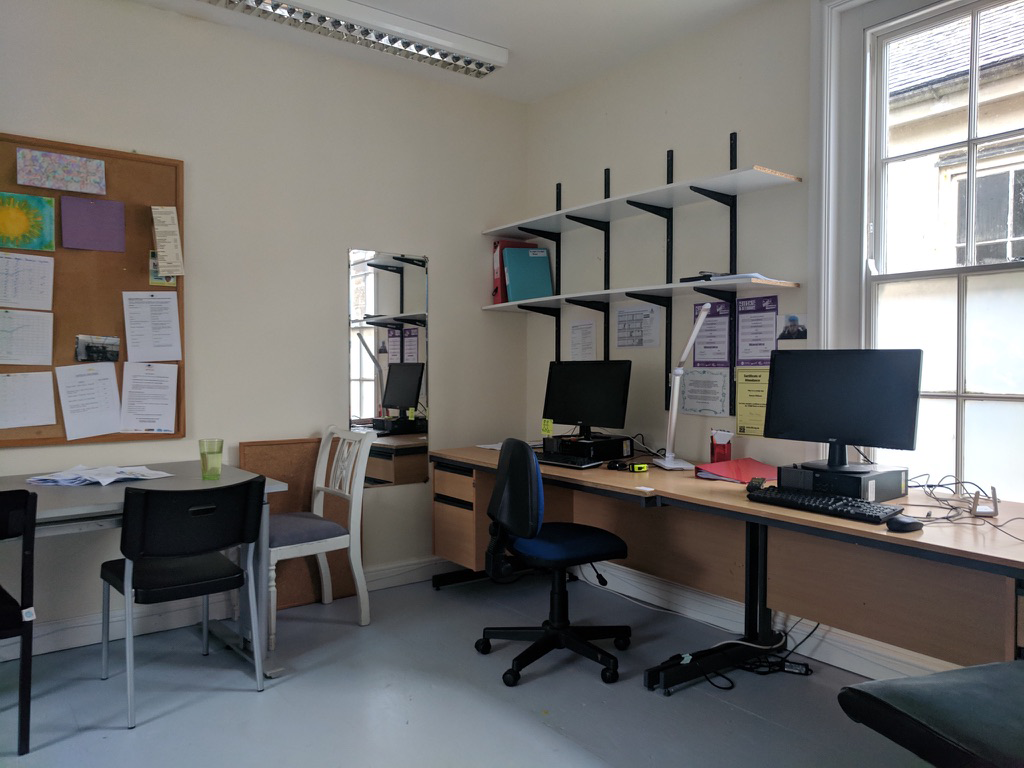
\includegraphics[width=1\linewidth]{Images/3/seabird.png}
    \caption{The view from my desk in Seabird's offices.}
    \label{fig:seabird}
\end{figure}

We arrived at a damp building that had once been a school, then a SureStart centre, and which was now living an in-between life: occasionally an events space, occasionally empty. Despite being hosted by the local authority, the event mostly consisted of a lecture from one particular organisation—SafeFutures. SafeFutures were an organisation that had been recently founded in response to constantly-growing Child and Adolescent Mental Health Services (CAMHS) waiting lists; their remit was to do something different, develop new practice, and then eventually, try to make systems change within the space of children and young people's mental health. The event had primarily been marketed as being about e-safety, though, so I was beginning to feel a little confused. I understood the relationship between digital safety and (in particular, child and adolescent) mental health, but I noticed the beginning of a slippage occurring: this was not the event I had thought it was going to be, but this seemed a very familiar set of interactions to everyone around me. I sat back and paid attention. 

As the event went on, the focus on e-safety became increasingly about the need for children and young people to become resilient. Resilience is frequently thrown around in work with children and young people perceived to be vulnerable, as a way to refer to a young person's ability to `bounce back' from something difficult. Whilst it is true that children and young people who score as resilient on outcomes frameworks tend to have better life experiences, this tends to miss the point that resilience is a capacity that is developed within a community: it originates from ecological and systems work, focusing on the ability of a system to return to a equilibrium state from crisis. Like much of what the person leading the session from SafeFutures was saying, this focus on resilience \textit{does} have a basis in research—just not necessarily in the way that it was being deployed. Individual people cannot become resilient without the system around them becoming more resilient; individual resiliency depends directly on a system's resiliency. 

I begin to notice that the person delivering the lecture followed a pattern in his presentation of information. He would give an incredibly complex explanation of a concept—like resilience, or trauma—and then make out that it was far too hard to understand, proceeding to give the audience an incredibly simplified version that missed a lot of the important nuance. He proceeded to give the most complex definition of resilience I've ever heard, then disregarded it in favour of explaining that we can think of resilience like Tigger (from Winnie the Pooh; he bounces back) or like Iron Man (able to push things away, and call on his friends for help when he needs it). Neither of these account for the systems-level adaptations necessary for the development of resilience. The only time he didn't perform this pattern was in his explanation of the neurobiology of a child's developing brain. He used specialist terms with no explanation. He described in minute detail the way that Adverse Childhood Experiences impact neurological development. He cited research for the only time in his lecture to support his argument. It appeared to me to be a kind of legitimacy work, of justifying the takeaway message that "young people need to be more resilient (in both the physical and digital worlds), otherwise their Adverse Childhood Experiences might affect their neurological development". There was no room for contestation or even questions, which struck me as odd for an event billed as a `learning lunch'.

After the event, Tina and I catch up. She tells me that she didn't think the event was particularly good, and I'm briefly encouraged, thinking that she might have had a similar experience to me—before she explains that it was because she'd heard the same presentation four times before. Here, the slippage emerged. Even if you were hesitant the first time you heard some of these concepts, by the fourth time, it will have made some kind of lasting imprint. Although they're marketed as events to disseminate best practice, these learning lunches begin to function as a mechanism of control: shaping the space of what is considered legitimate in the world of youth and social work. 

Before the presentation, Tina and I had been speaking about resilience, and she had described it in almost identical words as the person from SafeFutures did later in the presentation, as bouncing back, and calling on others. She described some training she went on recently to become a trauma-informed practitioner, in which she saw "a photograph of the DNA of people with Adverse Childhood Experiences". According to her, the photo showed the DNA "coming apart at the ends", beginning to fray. This isn't how the epigenetics of trauma works. Yes, traumatic experiences leave biomarkers on individual's DNA that may alter the mechanism of expressing that DNA, but the expression of genetic traits cannot be inferred through DNA structure alone. It begins to become clear to me that a certain simplified version of neurobiological research is being deployed in youth work settings, disseminated as `best practice' and delivered in a way that doesn't give space to critically assess the information. Practitioners who have no specialist scientific training—and who have no real \textit{need} for scientific training—are being asked to learn and work with complex science that is being misrepresented through simplification. Whether it is fraying DNA or Tigger bouncing back, I began to realise that understanding the neurobiology of trauma and attachment was becoming a necessary endeavour for youth workers working with young people perceived to be vulnerable. The people I was working with needed to have a clear, measurable, and scientific justification for \textit{why} their work is important.

\section{Conclusion}

In this chapter, I introduced The Charity, a composite entity that works with children and young people across the United Kingdom, and three of their projects: Small Steps, Building Bridges, and Seabird. I introduced significant people in these projects, such as Shelly and Colin; Michael, Karen and Mandy; and Dan, Tina, Trudy, Jake, and Tessa. Through three vignettes charting the slippages I experienced in my time with these organizations, I have presented the journey that I went on at the beginning of this research. Importantly, these slippages showed me how organizations that have values grounded in being young person-led are directed away from this focus. Small Steps showed me how organizations begin to focus more on the acquisition of further funding than delivering work they were already funded to do; Building Bridges showed me how even the most young people-led and `innovative' managers can have their hands tied by organizational constraints; and Seabird showed me how these practices begin to take hold, disseminated through events for `best practice' whilst deploying increasingly complex justifications for why their work with young people is valuable. In the following chapters, I will reflect on the experiences of young people and frontline workers in The Charity, and question how their experiences are facilitated by the network of power that sustains these slippages.